%!TEX root = ../../Main.tex
\graphicspath{{Chapters/Indledning/}}
%-------------------------------------------------------------------------------

\chapter{Simple linear regression / Multiple linear regression}

The simple Linear Regression approach is a quick and simple method for predicting a response Y based on X. The linear model is used to give an idea of the relationship between to dataset. For this to be true an assumption that the two variables have a linear relationship is needed. The mathematical representation of this can be seen below.

\begin{equation} \label{eq:Linear_Regression_eq}
	\begin{split}
		Y & \approx \beta_0 + \beta_1 X
	\end{split}
\end{equation} 

\cref{eq:Linear_Regression_eq} can also be seen as "Regressing Y onto X". As an example the dataset Advertising.csv contains sales on a certain product and advertisement money spent on certain media platforms. X represents TV advertising and Y represents sales. It is the possible to regress sales onto TV. This is expressed as:

\begin{equation} \label{eq:Linear_Regression_eq_sales}
\begin{split}
sales & \approx \beta_0 + \beta_1 TV
\end{split}
\end{equation} 


The two constants $\beta_0$ and $\beta_1$ represents the intercept (Where it intercepts the y-axis) and slope of the linear model. These constant needs to be predicted and when they have we will end out with a linear model that fits our data.

\section{Predict $\beta_0$ and $\beta_1$}
In the Advertising.csv dataset a number of observations (n = 200) have been made on amount of advertisements for tv, radio, newspaper and the corresponding sales. The advertisement data can be seen on \cref{fig:Advertisement_data}.

\begin{figure}[H]
	\centering
	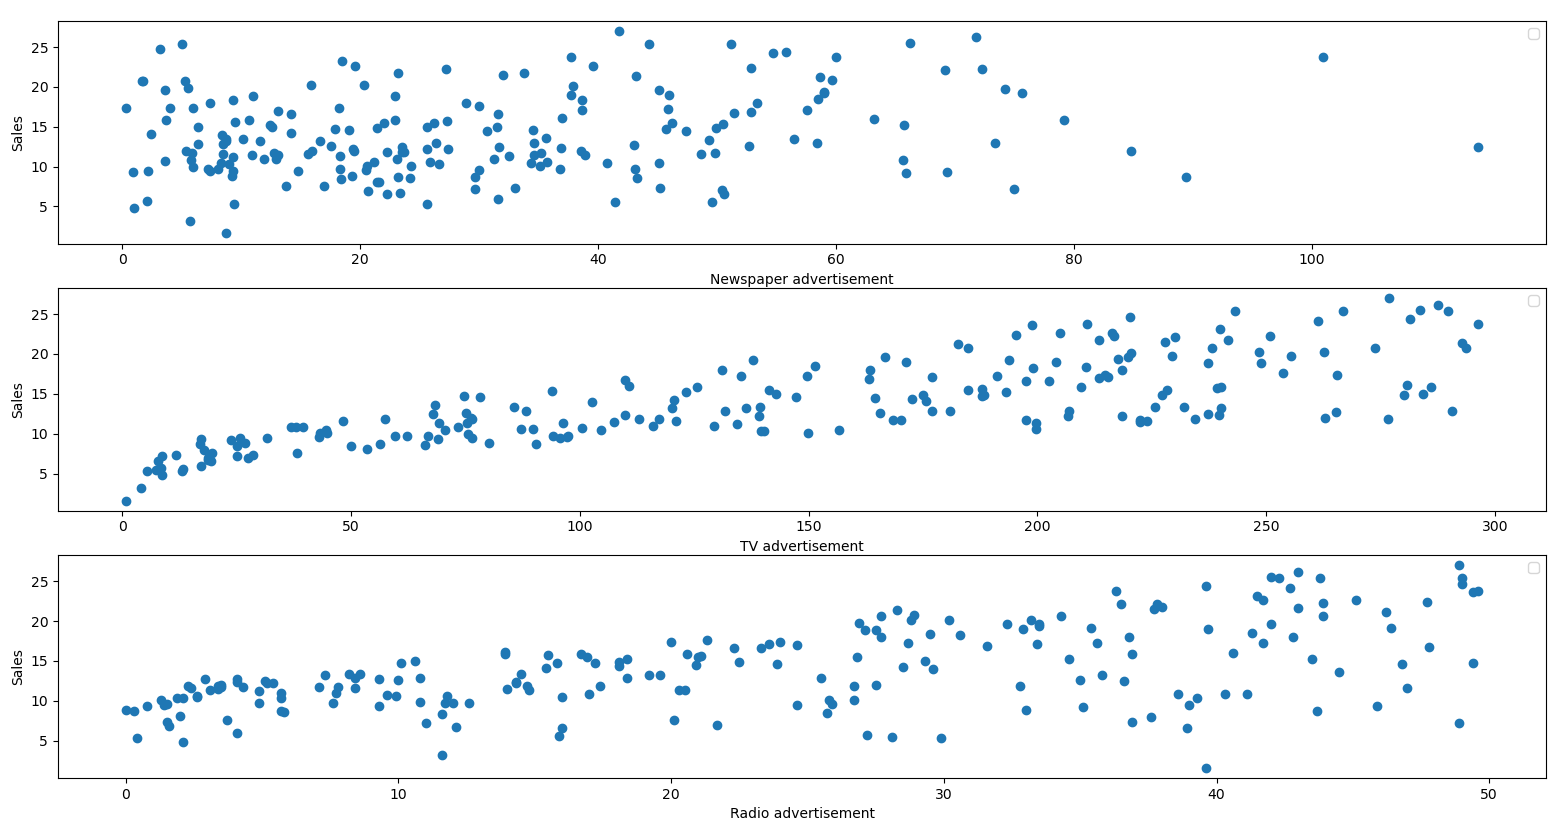
\includegraphics[width=\textwidth]{Img/Advertisement_data.PNG}
	\caption{Advertisement data}
	\label{fig:Advertisement_data}
\end{figure} 

To estimate $\beta_0$ and $\beta_1$ we need to introduce RSS which is the \textit{residual sum of squares}. RSS is the difference or error between observed response value and predicted response value that is predicted by our linear model. On \cref{fig:TV_linear_reg} a linear model is put on top of the TV advertisement data. The RSS is the summed value of the difference between the red points to the blue line. We want this value to b as low as possible to get the most accurate model. 

\begin{figure}[H]
	\centering
	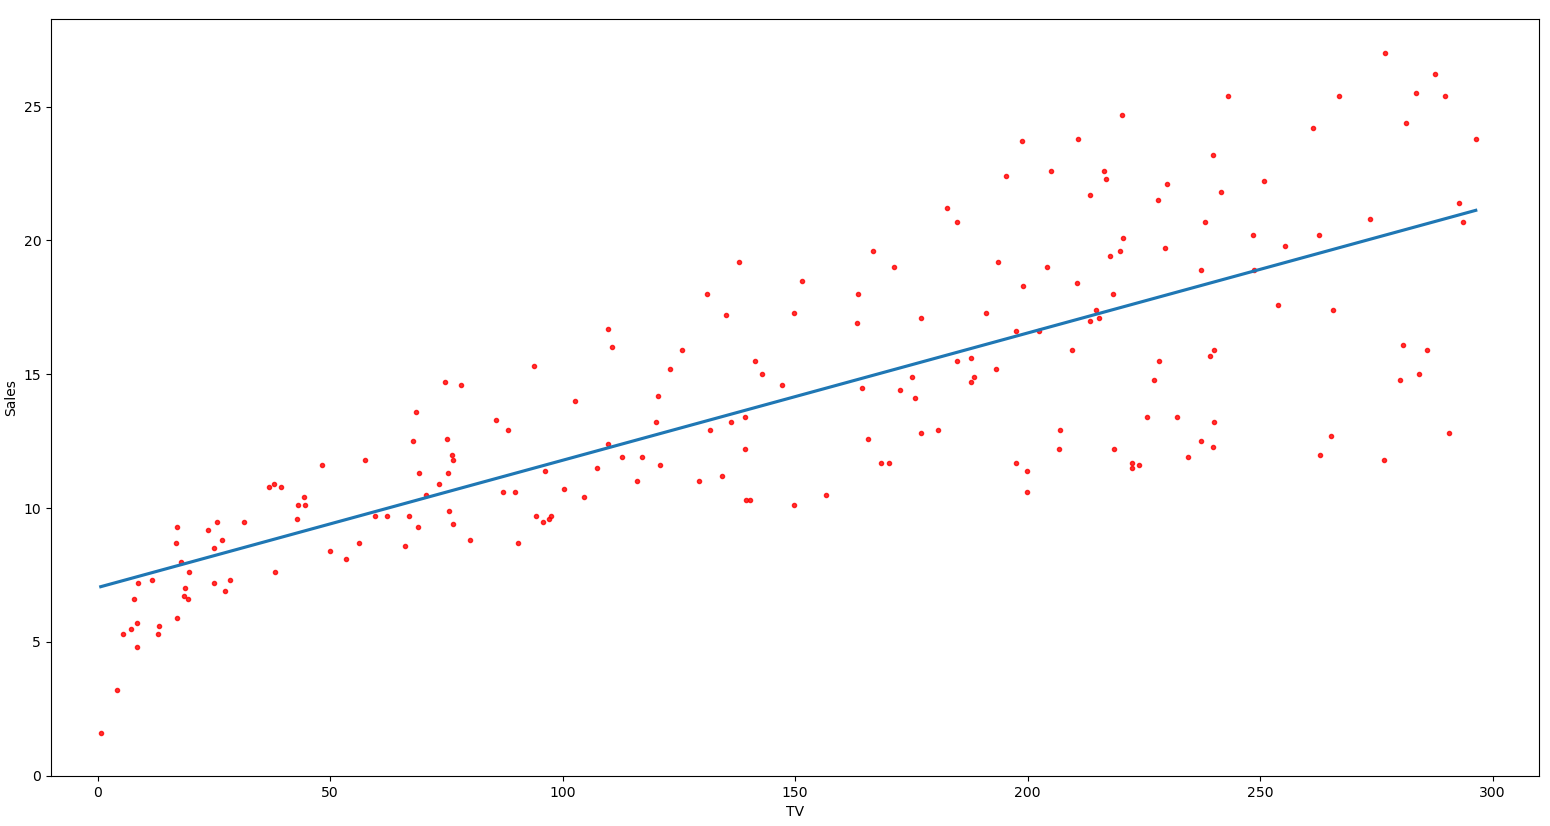
\includegraphics[width=\textwidth]{Img/Regplot_tv.PNG}
	\caption{Linear regression on TV advertisement}
	\label{fig:TV_linear_reg}
\end{figure} 

We can define the RSS value as:


\begin{equation} \label{eq:RSS}
\begin{split}
RSS = e_{1}^{2}+e_{2}^{2}...e_{n}^{2} \\
where \\
e = y_{i}-\hat{y}
\end{split}
\end{equation} 

This means that to get to a final method we need to minimize RSS. Some calculus shows that these minimizers are:

\begin{equation} \label{eq:RSS_e}
\begin{split}
\hat{\beta_1}=\frac{\sum_{i=1}^{n}(x_{i}-\overline{x})(y_{i}-\overline{y})}{\sum_{i=1}^{n}(x_{i}-\overline{x})^{2}} \\
\beta_0=\overline{y}-\beta_1\overline{x} \\
\textbf{where} \\
\overline{y}=\dfrac{1}{n}\sum_{i=1}^{n}y_{i} \\
\textbf{and} \\
\overline{x}=\dfrac{1}{n}\sum_{i=1}^{n}x_{i} 
\end{split}
\end{equation} 

This method of estimating the constants have been used on \cref*{fig:TV_linear_reg}. How this is done can be seen on the code snippet below.

\begin{lstlisting}[language=Python]
x_mean = get_mean(x_data)
y_mean = get_mean(y_data)

num = 0
den = 0

for i in range(len(x_data)):
num += (x_data[i]-x_mean)*(y_data[i]-y_mean)
den += (x_data[i] - x_mean) ** 2

b1_hat = num/den
b0_hat = y_mean-b1_hat*x_mean

return b0_hat, b1_hat
\end{lstlisting}

$\beta_0$ and $\beta_1$ is estimated to 7.03 and 0.04 respectively for the TV advertisement data.

There will always be an error of some sort when estimating this linear model. Because of this we can add a error constant to \cref{eq:Linear_Regression_eq}. The error constant (epsilon) is generated based on a gaussian distribution with a mean of 0. The equation will look as the following:

\begin{equation} \label{eq:linear_reg_e}
\begin{split}
Y & \approx \beta_0 + \beta_1 X + \epsilon
\end{split}
\end{equation} 

\section{Multiple linear regression}
Simple linear regression is a great to see the response of a single predictor variable. However there are times where it would be beneficial to have multiple predictor variables. Instead of having only a 1-dimensional regression line we can with multiple linear regression have a many-dimensional regression line (plane for 2D, cloud for 3D).

In simple linear regression we had an intercept constant, $\beta_0$ and a slope constant $\beta_1$. In this model we essentially have the same plus some extra slope constant and predictor variables. This can be seen on \cref{eq:Multiple_lin_reg}.



\begin{equation} \label{eq:Multiple_lin_reg}
\begin{split}
Y = \beta_0 + \beta_1 X_{1} + \beta_2 X_{2}+...+\beta_{p}X_{p}+\epsilon
\end{split}
\end{equation}

If we fit this equation to out advertisement example we would get:

\begin{equation} \label{eq:RSS_multi}
\begin{split}
\textbf{sales} = \beta_0 + \beta_1 \textbf{TV} + \beta_2 \textbf{Radio}+\beta_2 \textbf{Newspaper}+\epsilon
\end{split}
\end{equation}

\subsection{Estimating the regression constants}
To estimate the constants we do same as in the simple regression method with some changes. We still try to minimize the RSS value, but since there are more constants the RSS value is calculated with the equation \cref{eq:RSS_multi_extended}. However to estimate the constants itself the use of a python package has been used. Sklearn has a regression module that can estimate our constants. This can be seen in the codes snippet further down in this chapter.

\begin{equation} \label{eq:RSS_multi_extended}
\begin{split}
 RSS = \sum_{i=1}^{n}(y_{i}-\hat{y}_{i})^{2} \\
	= \sum_{i=1}^{n}(y_{i}-\hat{\beta_0}-\hat{\beta_1}x_{i1}-\hat{\beta_2}x_{i2}-...-\beta_p x_{ip})^{2}
\end{split}
\end{equation}

When using two predictor variables the regression line becomes a plane. On \cref{fig:Multi_reg_plane} the regression pane when using TV and Radio as predictor variables is shown. The plane is placed in a way such that the RSS value is as low as possible. 

\begin{figure}[H]
	\centering
	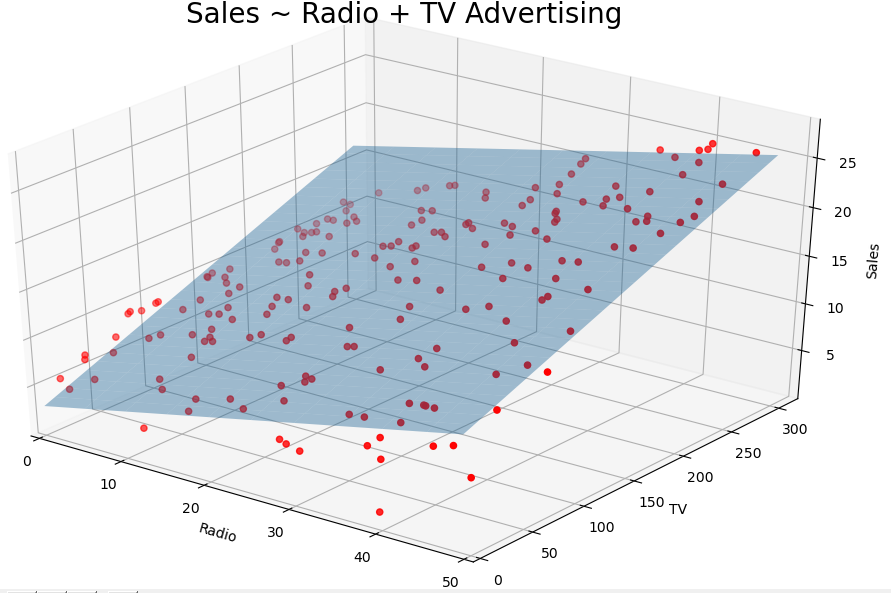
\includegraphics[width=\textwidth]{Img/Multi_reg_plane.PNG}
	\caption{The regression pane with TV and Radio as predictor variables}
	\label{fig:Multi_reg_plane}
\end{figure} 

The code for making the regression plane is listed below:

\begin{lstlisting}
# Multiple Regression
regr = skl_lm.LinearRegression()

X = advertising[['Radio', 'TV']].values
y = advertising.Sales

# Fitting data to estimate constants.
regr.fit(X, y)

# Make it so that the plane fits all points
Radio = np.arange(0, 50)
TV = np.arange(0, 300)


B1, B2 = np.meshgrid(Radio, TV, indexing='xy')
Z = np.zeros((TV.size, Radio.size))

for (i, j), v in np.ndenumerate(Z):
# The response on TV and Radio
Z[i, j] = (regr.intercept_ + B1[i, j] * regr.coef_[0] + B2[i, j] * regr.coef_[1])
\end{lstlisting}


